\chapter{Distance education}

Distance education is not only a phenomenon of the few last decades, but can be traced at least back to the 18th century, when Caleb Phillipps posted an advertisment called ``Teacher of the New Method of Short Hand'' in Boston Gazette, saying ``Persons in the Country desirous to Learn this Art, may by having the several Lessons sent weekly to them, be as perfectly instructed as those that live in Boston.'' \cite{1}

With the development of the Internet and its general accessibility in the developed world, providing distance education has become much easier and has spread widely. In some countries tuition rates are high and young people take loans. This topic is covered in a fitting way by John Oliver in his show \cite{2}. The flexibility and low cost of distatnce education over the Internet gives people, who wouldn't be otherwise able to attend a traditional university, an opportunity to gain knowledge and train skills from their homes \cite{3} spending much less money or even for free.

Students in the deveopling world are also taking the advantage of educational content available on the Internet. Several of the top U.S. universities, like Harvard, Stanford or MIT, put some of their materials on so called MOOCs (Massive Open Online Course) like Coursea, edX or Udacity. This content is then available to anyone with a computer and Internet connection and knowledge of the language. An great example is \textit{Kepler} - non profit university project in Rwanda \cite{5}. The goal of this project is to ``provide an American-accredited degree, a world class education, and a clear path to good jobs for thousands of students for around \$1,000 tuition per year.'' \cite{6}

A concept of teaching often refered to as \textit{Flipped Classroom} uses distance education. The idea is to let students study lecture materials at home at their own pace and then apply the things at school the next day by doing activities to illustrate the concepts. The teacher can then help them or explain details here in person. These materials are often in the form of videos either from an open source, like the Khan Academy, or created by the teacher himself.

\section{Current systems}
In the next few paragraphs I will try to pick some of current distance education services and tools available on the Internet. This list is not complete and is only meant to give the reader a notion of available technologies and their paradigms, on which the project of Vector Screencast is based.

\subsection{Coursera}
The mission of \textit{Coursera} is to ``provide universal access to the world’s best education.'' \cite{9} Anyone can, for free, go through materials published by universities and other organizations aimed at education.

Courses at Coursera consist mainly of video lectures commonly with a transcript and a presentation document attached to. These videos can be viewed directly in web browser on demand or downloaded to user's computer. After studying the materials, students can submit assignments' solutions and take quizes and receive a Verified Certificate for the accomplishment of the course. These certificates are not free.

Most of the courses are in English and only a few of the courses are also translated into other languages. It is not possible for everyone to publish his materials through Coursera.

\subsection{Youtube.com}
\textit{Youtube.com} \cite{10} is not an educational service by design. Youtube allows people to create their own channels and upload their video content to share it with other Internet users for free.

Youtube was launched in 2005 and has became one of the most frequently visited websites on the Internet according to Alexa Internet \cite{11}. Uploading video to Youtube is free, advertisment is displayed to the user while watching videos though.

The ease of making original-created videos available and the wide audience makes Youtube a perfect place for all individuals and organizations, who want to share their ideas or any video materials. Many educational channels can be found here, for example \textit{Numberphile} \cite{12}, \textit{Veritasium} \cite{13}, and \textit{Khan Academy} \cite{14}.

Youtube videos can be viewed only online in a web browser or a specialized mobile app. There are only unofficial tools for downloading these videos.

The form and content of the video is practicaly unlimited, as long as does not violate the terms of the service. The maximum file size of a video is 128 GB in size and 11 hours in length. To upload larger or longer videos, user must split them into several parts. Video can have a text description which might contain the transcription of the video content and any subtitles can be attached to a video. Youtube also downscales videos to multiple resolutions so they can be viewed with a low speed Internet connection.



\subsection{Moodle}
\textit{Moodle} \cite{7} is an open-source project used by millions of users \cite{8} providing a robust tool for creating custom learning materials and providing them to students. The source code of Moodle can be downloaded and deployed it any server. Teachers then publish their materials and resources for students or for assigning homework.




\subsection{Educreations and ShowMe}
\textit{Educreations} is a service for creating and sharing educational videos similar to Khan Academy videos. The idea is that teachers create a their own videos by drawing onto a digital whiteboard and then share these videos with their classes.

Educreations is designed for an iPad device, but can be used also as a web application from any web browser, that supports Adobe Flash Player. Web application supports playing and recording and video player can be easily embeded into any website. Content of the video is scaled appropriately to the output screen and is drawn smoothly.

There is a free variant, which is limited. For more storage capacity and advanced tools, users must pay monthly fees. The software is proprietary and is is the file format of the video.

\textit{ShowMe} \footnote{http://www.showme.com/} is a very similar service. An iPad app is available for recording and viewing videos. Recorded videos can then be played in a web browser, but not recorded. Pricing is very similar to Educreations.

Both ShowMe and Educreations of these services target mainly on tablets. The advantage of tablets is their touchscreen, which can be used for drawing in a natural way with fingers or a special stylus.



\subsection{Khan Academy}
A similar service to Coursera is \textit{Khan Academy}. Khan Academy originated in 2003 when it's founder, Salman Khan, began tutoring his cousin over an instant messenger via drawing pictures with a computer mouse. Salman then started to record these videos and put them on his Youtube channel, so someone could watch them later. This channel became the base of Khan Academy.

Khan Academy became known and has grown a lot, but the style of Khan Academy videos remained the same. A person draws lines and diagrams using a bitmap editor on his computer and talks about the subject aloud while recording his computer screen and recording his voice using a microphone. These videos are then uploaded to Youtube and embedded on the Khan Academy website \cite{14}. Apart form the video lectures, the website also contains exercises and quizes to encourage students in learning. The pace of the lesson depends on the student. He can pause the videos or watch them multiple times before continuing with the lesson~\ref{fig:khan-screen}.

Most of the videos are recorded in English, but many of the videos are translated into other languages - by replacing the audio track with a different one or with subtitles.

One of the projects working on the localization of Khan Academy videos is a czech branch called Khanova Škola\cite{15}.

\begin{figure}
	\centering
	%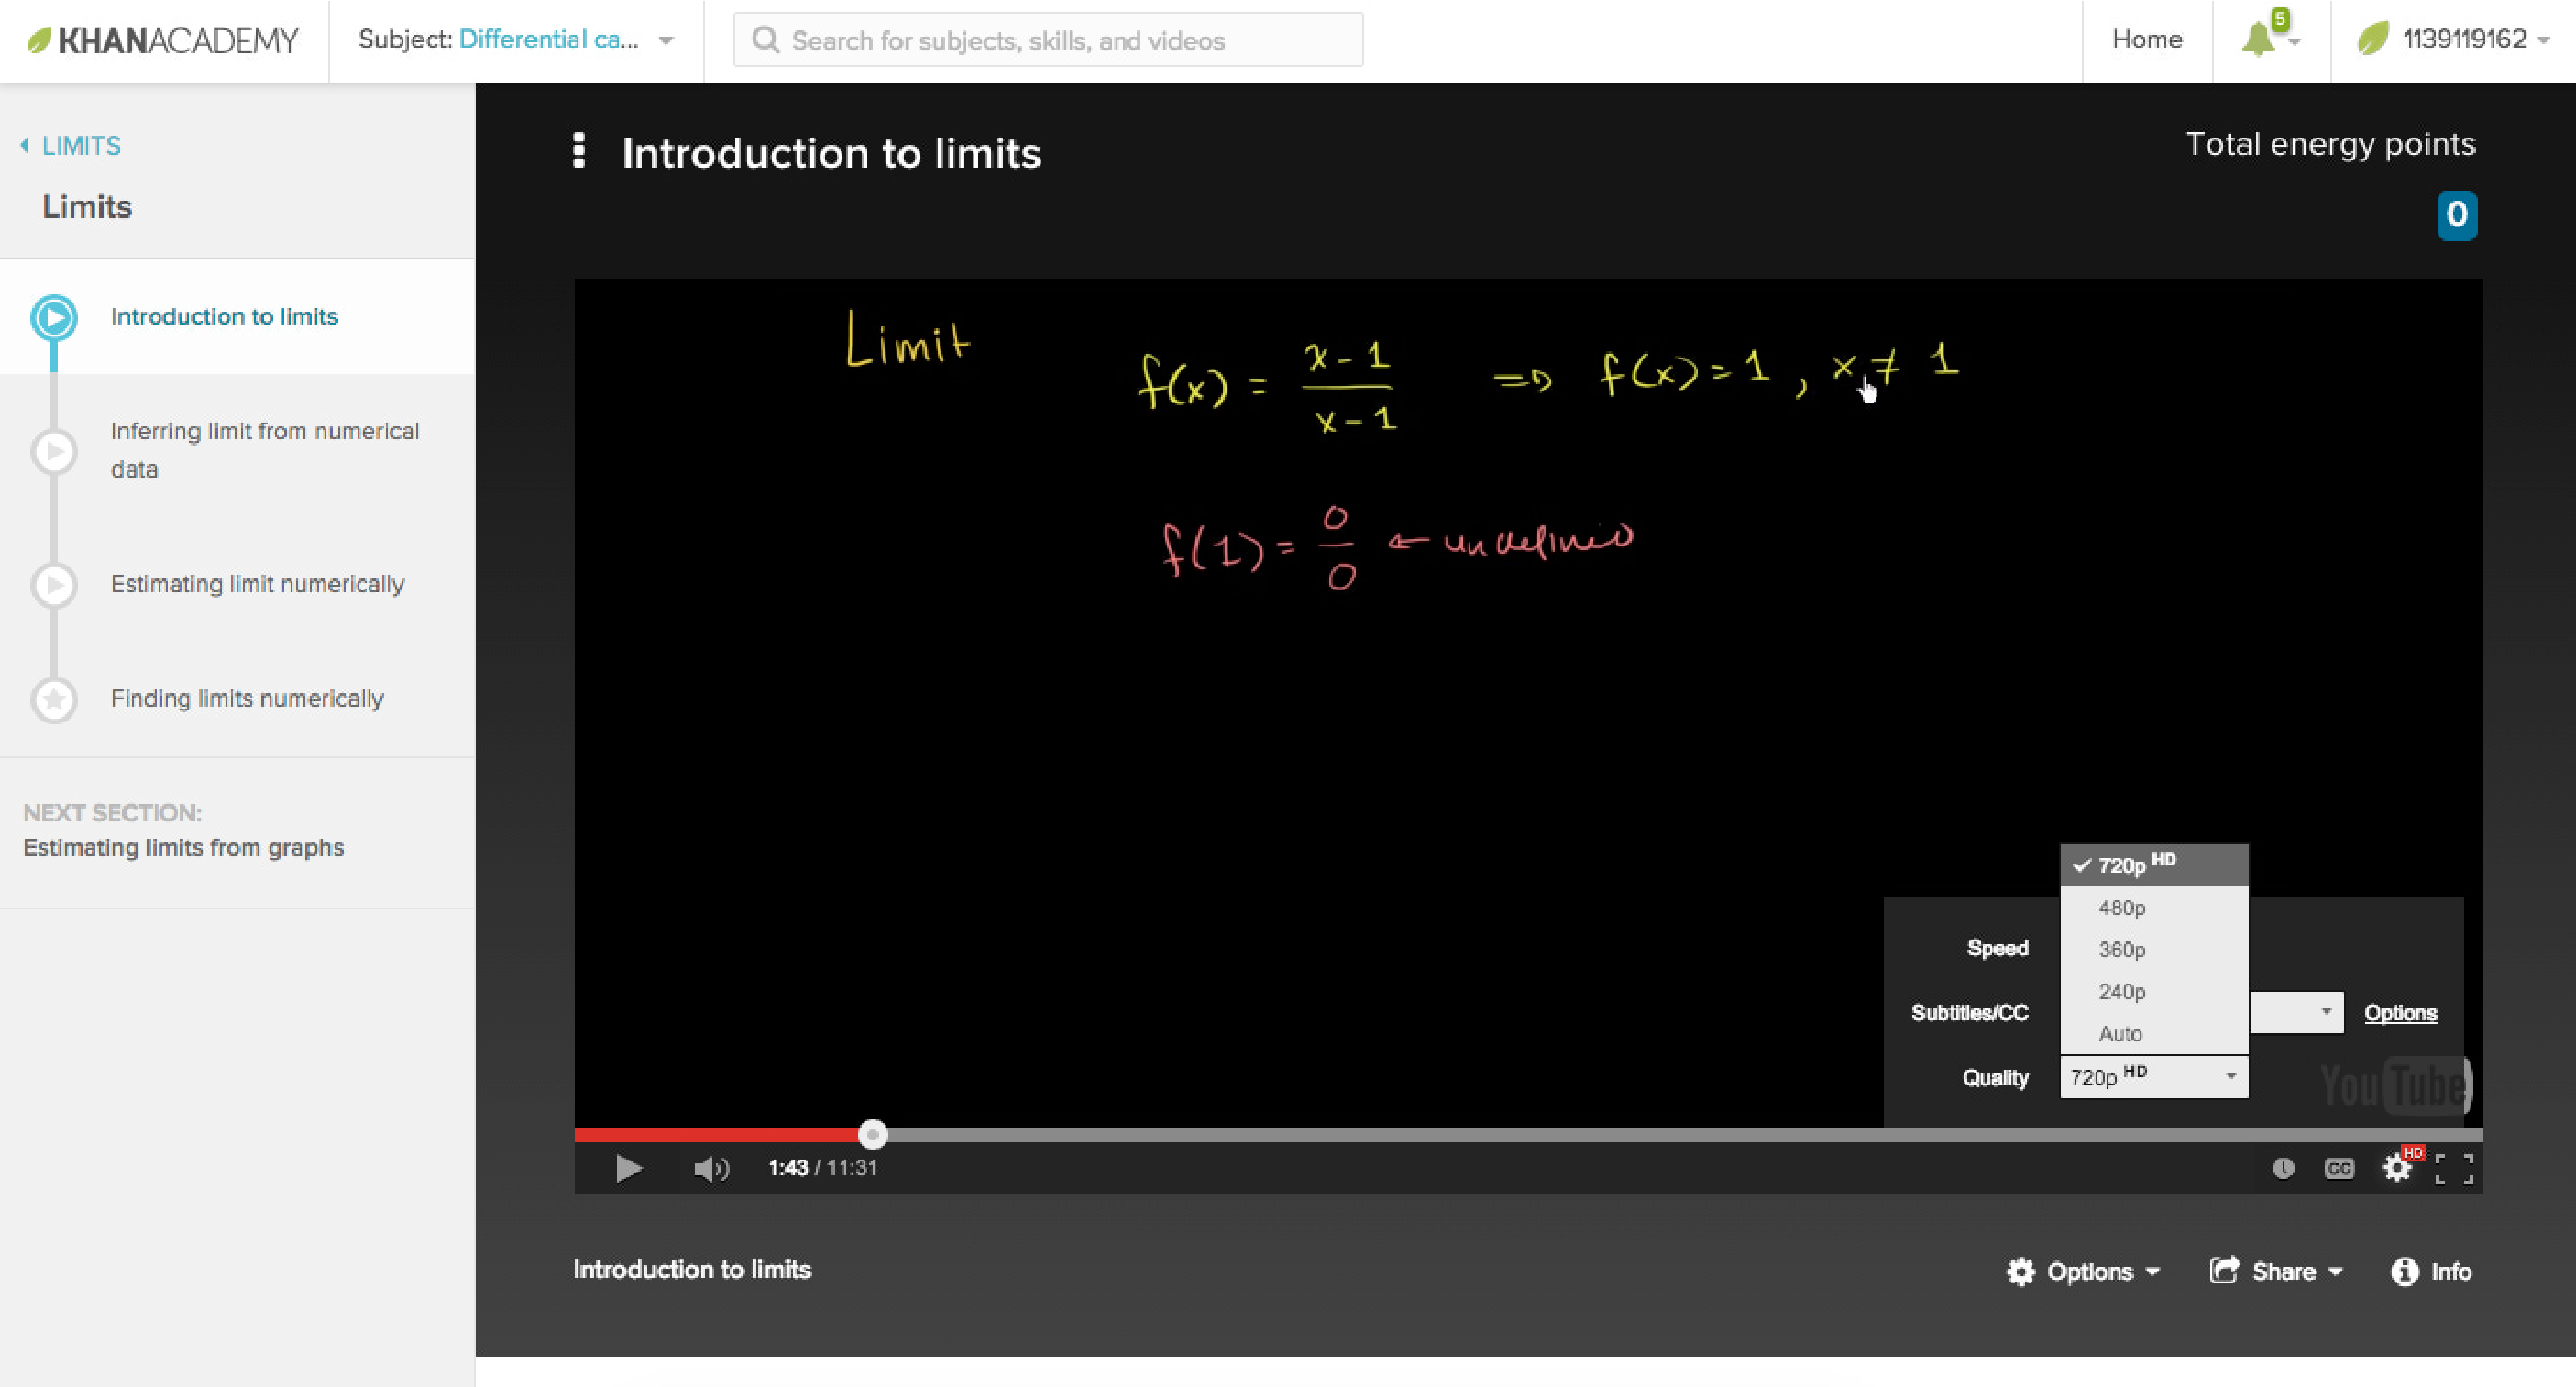
\includegraphics[width=30mm,natwidth=1348,natheight=726]{../img/khan-academy-screenshot.png}
	\caption{Khan Academy lesson}
	\label{fig:khan-screen}
\end{figure}